\documentclass[tikz]{standalone}


\usetikzlibrary{math,decorations.pathreplacing,calc,decorations.markings}
\tikzset{->-/.style={decoration={
			markings,
			mark=at position {0.5*\pgfdecoratedpathlength+.5*3pt} with {\arrow{>}}},postaction={decorate}}}
\tikzset{-<-/.style={decoration={
			markings,
			mark=at position {0.5*\pgfdecoratedpathlength+.5*3pt} with {\arrow{<}}},postaction={decorate}}}

\begin{document}
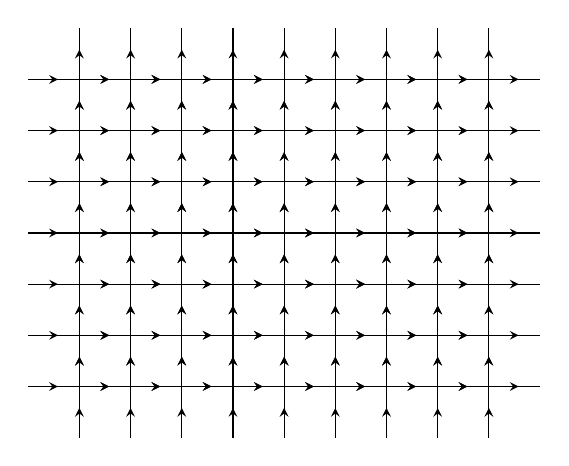
\begin{tikzpicture}[>=stealth, scale=0.65]
	\foreach \i in {-4,...,4} {
		\foreach \j in {-3,...,3} {
			\draw[->-] (\i,\j) -- ({\i+1},{\j});
			\draw[->-] (\i,\j) -- ({\i},{\j+1});
			\draw[->-] ({\i-1},\j) -- (\i,\j);
			\draw[->-] (\i,{\j-1}) -- (\i,\j);
		};
	};
\end{tikzpicture}
\end{document}